\lab{QR 2: Applications}{Applications of the QR Decomposition}
\label{lab:qr-applications}
\objective{Because of its numerical stability and convenient structure, the QR decomposition is the basis of many important and practical algorithms.
In this lab, we introduce linear least squares problems, tools in Python for computing least squares solutions, and two fundamental eigenvalue algorithms.
\\ \indent As in the previous lab, we restrict ourselves to real matrices and therefore use the transpose in place of the Hermitian conjugate.}

\section*{Least Squares} % ====================================================

A linear system $A\x = \b$ is \emph{overdetermined} if it has more equations than unknowns.
In this situation, there is no true solution, and $\x$ can only be approximated.

The \emph{least squares solution} of $A\x = \b$, denoted as $\widehat{\x}$, is the ``closest'' vector to a solution, meaning it minimizes the quantity $\|A\widehat{\x} - \b\|_2$.
% \footnote{The choice of the 2-norm is significant.}
In other words, $\widehat{\x}$ is the vector such that $A\widehat{\x}$ is projection of $\b$ onto the range of $A$, and can be calculated by solving the \emph{normal equation}:%
\footnote{See Volume 1 Chapter 3 for a formal derivation of the normal equation.}
\[A\trp A\widehat{\x} = A\trp \b\]

If $A$ is full rank, which it usually is in applications, its QR decomposition provides an efficient way to solve the normal equation.
Let $A = \widehat{Q}\widehat{R}$ be the reduced QR decomposition of $A$, so $\widehat{Q}$ is $m \times n$ with orthonormal columns and $\widehat{R}$ is $n \times n$, invertible, and upper triangular.
Since $\widehat{Q}\trp \widehat{Q} = I$, and since $\widehat{R}\trp$ is invertible, the normal equation can be reduced as follows (we omit the hats on $\widehat{Q}$ and $\widehat{R}$ for clarity):
%
\begin{align}
\nonumber
A\trp A\widehat{\x} &= A\trp \b \\ \nonumber
(Q R)\trp Q R  \widehat{\x}
&= (Q R)\trp \b \\ \nonumber
 R\trp Q\trp Q R  \widehat{\x}
&=  R\trp Q\trp \b \\ \nonumber
 R\trp R \widehat{\x}
&=  R\trp Q\trp \b \\
 R \widehat{\x}
&= Q\trp \b \label{eq:normal-equation-via-qr}
\end{align}

Thus $\widehat{\x}$ is the least squares solution to $A\x=\b$ if and only if $\widehat{R}\widehat{\x} = \widehat{Q}\trp\b.$
Since $\widehat{R}$ is upper triangular, this equation can be solved quickly with back substitution.

\begin{problem} % Solve the normal equations with QR.
Write a function that accepts an $m \times n$ matrix $A$ of rank $n$ and a vector $\b$ of length $n$.
Use the QR decomposition and Equation \ref{eq:normal-equation-via-qr} to solve the normal equation corresponding to $A\x = \b$.

You may use either SciPy's QR routine or one of your own routines from the previous lab.
In addition, you may use \li{la.solve_triangular()}, SciPy's optimized routine for solving triangular systems.

\label{prob:lstsq-via-qr}
\end{problem}

\subsection*{Using Least Squares to Fit Curves to Data} % ---------------------

The least squares solution can be used to find the best-fit curve of a chosen type to a set of points.
This is perhaps the most common application of least squares.

\subsubsection*{Fitting a Line} % - - - - - - - - - - - - - - - - - - - - - - -

Consider the problem of finding the line $y = mx + b$ that best fits a set of $n$ points $\{(x_k, y_k)\}_{k=1}^n$.
Ideally, we seek $m$ and $b$ such that $y_k = mx_k + b$ for all $k$.
The following linear system simultaneously represents all of these equations.
%
\begin{equation}
\left[\begin{array}{cc}
x_1 & 1 \\
x_2 & 1 \\
x_3 & 1 \\
\vdots & \vdots \\
x_n & 1
\end{array}\right]
\left[\begin{array}{c} m \\ b \end{array}\right]
=
\left[\begin{array}{c} y_1 \\ y_2 \\ y_3 \\ \vdots \\ y_n \end{array}\right]
\label{eq:linear-least-squares}
\end{equation}
%
Note that $A$ has rank $2$ as long as not all of the $x_k$ values are the same.

Because this system has two unknowns, it is guaranteed to have a solution if it has two or fewer equations.
However, if there are more that two data points, the system is overdetermined if any set of three points are not collinear.
We therefore seek a least squares solution, which in this case means finding the slope $\widehat{m}$ and $y$-intercept $\widehat{b}$ such that the line $y = \widehat{m}x+\widehat{b}$ best fits the data.

The following figure is a typical example of this idea where $\widehat{m} \approx \frac{1}{2}$ and $\widehat{b} \approx -3$.

\begin{figure}[H] % Linear regression example (without code).
    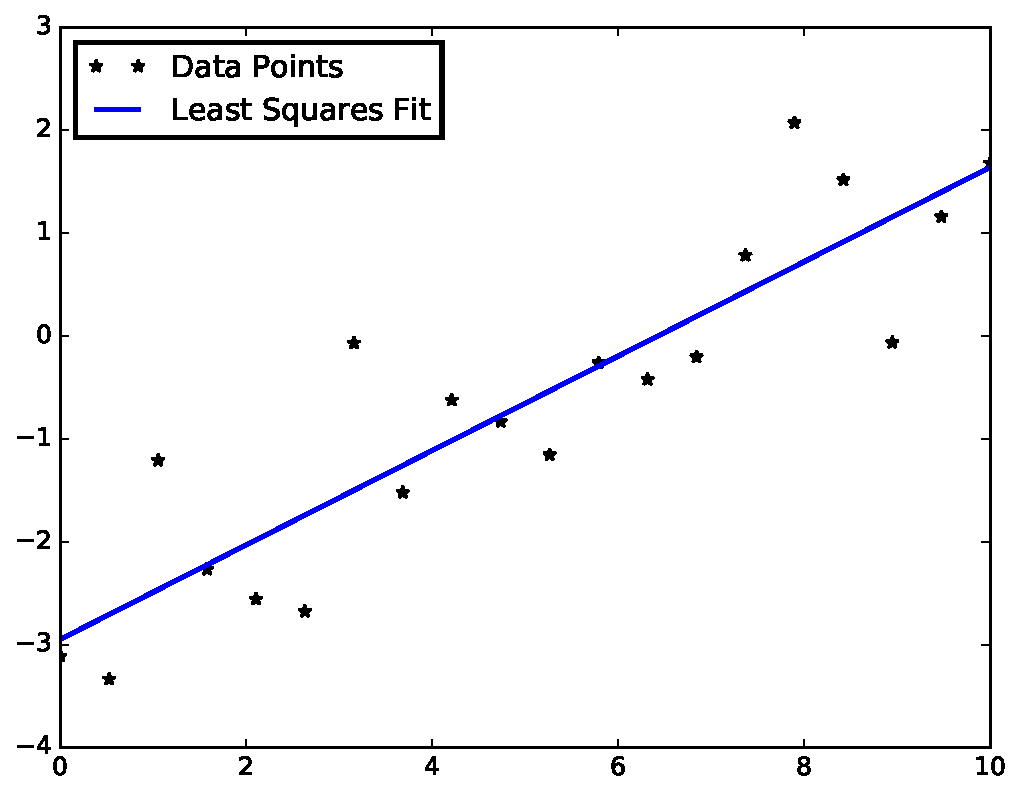
\includegraphics[width=.5\textwidth]{figures/line_fit_example.pdf}
\end{figure}

\begin{problem} % Linear regression of height vs weight.
The file \texttt{MLB.npy} contains measurements from over 1,000 recent Major League Baseball players, compiled by UCLA.\footnote{See \url{http://wiki.stat.ucla.edu/socr/index.php/SOCR_Data_MLB_HeightsWeights}.}
Each row in the array represents a different player; the columns are the player's height (in inches), weight (in pounds), and age (in years), in that order.

Find the least squares line that relates the height of the players to their weight (i.e., let height be the $x$ values and weight be the $y$ values).
%
\begin{enumerate}
    \item Construct the matrix $A$ and the vector $\b$ described by Equation \ref{eq:linear-least-squares}.\\
    (Hint: the functions \li{np.vstack()}, \li{np.column_stack()}, and/or \li{np.ones()} may be helpful.)
    \item Use your function from Problem \ref{prob:lstsq-via-qr} to find the least squares solution.
    \item Plot the data points as a scatter plot.
    \item Plot the least squares line with the scatter plot.\\
    (Hint: Make a new domain of $x$ values with \li{np.linspace()}, and use this domain to calculate $y = \widehat{m}x + \widehat{b}$.)
\end{enumerate}
\end{problem}

% \subsection*{Fitting a Polynomial} % - - - - - - - - - - - - - - - - - - - - -

\subsubsection*{Fitting a Circle} % - - - - - - - - - - - - - - - - - - - - - -

Now suppose we wish to fit a general circle to a data set $\{(x_k, y_k)\}_{k=1}^n$
Recall that the equation of a circle with radius $r$ and center $(c_1,c_2)$ is
\begin{equation}
\label{circle}
(x-c_1)^2 + (y-c_2)^2 = r^2.
\end{equation}

After expanding and rearranging this equation, we get
\begin{equation*}
\label{circle2}
2c_1x + 2c_2y + r^2 - c_1^2 - c_2^2 = x^2 + y^2.
\end{equation*}

To find $c_1$, $c_2$, and $r$ with least squares, we need \emph{linear} equations.
The equation above is not linear because of the $r^2$, $c_1^2$, and $c_2^2$ terms
Note that it is acceptable to have the $x^2$ and $y^2$ terms because the variables in this equation are $r$, $c_1$, and $c_2$, not $x$ and $y$.
We can do a trick to make this equation linear: create a new variable $c_3$ defined by $c_3 = r^2-c_1^2-c_2^2$.

For a general data point $(x_k, y_k)$, we get the linear equation
\begin{equation*}
2c_1x_k+2c_2y_k+c_3=x_k^2+y_k^2.
\end{equation*}
Thus, we can find the best-fit circle from the least squares solution to the matrix equation

\begin{equation}\label{equ:circle_fit}
\begin{pmatrix}
2 x_1 & 2 y_1 & 1\\
2 x_2 & 2 y_2 & 1\\
\vdots & \vdots & \vdots \\
2 x_n & 2 y_n & 1
\end{pmatrix}
\begin{pmatrix}
c_1\\
c_2\\
c_3
\end{pmatrix}=
\begin{pmatrix}
x_1^2 + y_1^2\\
x_2^2 + y_2^2\\
\vdots\\
x_n^2 + y_n^2
\end{pmatrix}.
\end{equation}
If the least squares solution is $\widehat{c_1}, \widehat{c_2}$, $\widehat{c_3}$, then the best-fit circle is
\[
(x-\widehat{c_1})^2 + (y-\widehat{c_2})^2 = \widehat{c_3}+\widehat{c_1}^2+\widehat{c_2}^2.
\]

As an example, we use least squares to find the circle that best fits the nine points found in Table \ref{table:circlepts}:
\begin{table}
\begin{tabular}{c||c|c|c|c|c|c|c|c|c}
$x$& 5  &-53 & -45 &  28 & 74 & -51 &  65 & 142 & 120 \\ \hline
$y$& 11 & 35 & 139 & 170 & -7 &  87 & -24 &  64 & 131 \\
\end{tabular}
\caption{Points used in example of fitting to a circle using least squares.}
\label{table:circlepts}
\end{table}

We enter them into Python as a $9\times 2$ array.

\begin{lstlisting}
>>> P = np.array([[5,11],[-53,35],[-45,139],[28,170],[74,-7],
                [-51,87],[65,-24],[142,64],[120,131]])
\end{lstlisting}

We compute $A$ and $b$ according to Equation \ref{equ:circle_fit}.

\begin{lstlisting}
>>> A = np.hstack((2*P[:,:1], 2*P[:,1:], np.ones((9,1))))
>>> b = P[:,:1]**2 + P[:,1:]**2
\end{lstlisting}

Then we use SciPy to find the least squares solution.

\begin{lstlisting}
>>> c1, c2, c3 = la.lstsq(A, b)[0]
\end{lstlisting}

We can solve for $r$ using the relation $r^2 = c_3+c_1^2+c_2^2$.

\begin{lstlisting}
>>> r = np.sqrt(c1**2 + c2**2 + c3)
\end{lstlisting}

A good way to plot a circle is to use polar coordinates.
Using the same variables as before, the equation for a general circle is $x=r\cos(\theta)+c_1$ and $y=r\sin(\theta)+c_2$.
With the following code we plot the data points and our best-fit circle using polar coordinates.
The resulting image is Figure \ref{fig:circle}.

\begin{lstlisting}
# In the polar equations for a circle, theta goes from 0 to 2*pi.
>>> theta = np.linspace(0, 2*np.pi, 200)
>>> plt.plot(r*np.cos(theta)+c1, r*np.sin(theta)+c2, '-')
>>> plt.plot(P[:,0], P[:,1], '*')
>>> plt.show()
\end{lstlisting}

\begin{figure}[H]
    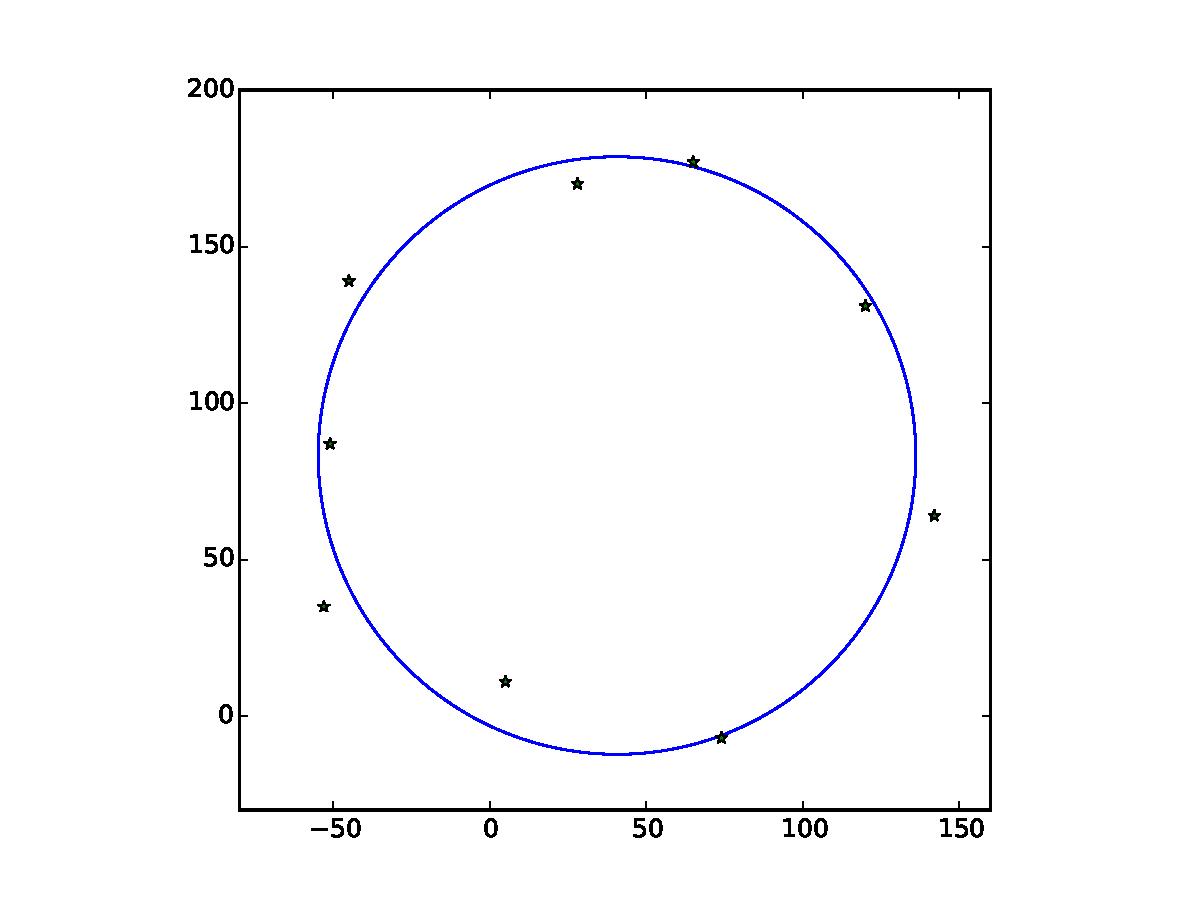
\includegraphics[width=\textwidth]{figures/circle.pdf}
    \caption{The graph of some data and its best-fit circle.}
    \label{fig:circle}
\end{figure}

\begin{comment}
\begin{problem}
Write a function \li{fitCircle} that does the following.
Load the \texttt{circlepts} array from \texttt{data.npz}.
This consists of two columns corresponding to the $x$ and $y$ values of a given
data set.
Use least squares to find the center and radius of the circle that best
fits the data.
Then plot the data points and the circle on the same graph.
The function should return nothing.
\end{problem}
\end{comment}

\begin{problem}
\leavevmode
\begin{enumerate}
\item Load the \texttt{ellipsepts} array from \texttt{data.npz}
This array has two columns corresponding to the $x$ and $y$ coordinates of some data points.
\item Use least squares to fit an ellipse to the data.
The general equation for an ellipse is
\[
ax^2 + bx + cxy + dy + ey^2 = 1.
\]
You should get  $0.087$, $-0.141$,  $0.159$, $-0.316$, $0.366$ for $a, b, c, d,$ and $e$ respectively
Generate a plot of the resulting curve and the data points used to produce the curve.
%\item Plot the data and your line on the same graph.
\end{enumerate}

We can plot our result using polar coordinates as we did when plotting the circle
Code for visualizing your best-fit ellipse is given below
Note this bit of code plots the curve and not the data points.

\begin{lstlisting}
    """Plots an ellipse of the form ax^2 + bx + cxy + dy + ey^2 = 1

    Input:
      X (array) - x-coordinates of all the data points.
      Y (array) - y-coordinates of all the data points.
      a,b,c,d,e (float) - the coefficients from the equation of an
                    ellipse of the form ax^2 + bx + cxy + dy + ey^2 = 1.
    """
    def get_r(a, b, c, d, e):
        theta = np.linspace(0,2*np.pi,200)
        A = a*(np.cos(theta)**2) + c*np.cos(theta)*np.sin(theta) + e*(np.sin(theta)**2)
        B = b*np.cos(theta) + d*np.sin(theta)
        r = (-B + np.sqrt(B**2 + 4*A))/(2*A)
        return r, theta

    r,theta = get_r(a,b,c,d,e)
    plt.plot(r*np.cos(theta), r*np.sin(theta), color = "r")
    plt.plot(X,Y,".", color = "b")
    plt.axes().set_aspect('equal', 'datalim')
    plt.show()
\end{lstlisting}

\end{problem}

\section*{Computing Eigenvalues} % ============================================

The eigenvalues of a matrix are the roots of its characteristic polynomial.
Thus, to find the eigenvalues of an $n \times n$ matrix, we must compute the roots of a degree-$n$ polynomial.
This is easy for small $n$.
For example, if $n=2$ the quadratic equation can be used to find the eigenvalues.
However, Abel's Impossibility Theorem says that no such formula exists for the roots of a polynomial of degree 5 or higher.

% TODO: get rid of this formal statement, as we provide no proof.
\begin{theorem}[Abel's Impossibility Theorem]
There is no general algebraic solution for solving a polynomial equation of degree $n\geq5$.
\label{thm:Abel}
\end{theorem}

Thus, it is impossible to write an algorithm that will exactly find the eigenvalues of an arbitrary matrix.
(If we could write such an algorithm, we could also use it to find the roots of polynomials, contradicting Abel's theorem.)
This is a significant result.
It means that we must find eigenvalues with \emph{iterative methods}, methods that generate sequences of approximate values converging to the true value.

% TODO: Decide whether or not to move this to Additional Material.
\subsection*{The Power Method} % ----------------------------------------------

There are many iterative methods for finding eigenvalues.
The power method finds an eigenvector corresponding to the \emph{dominant} eigenvalue of a matrix, if such an eigenvalue exists.
The dominant eigenvalue of a matrix is the unique eigenvalue of greatest magnitude.

To use the power method on a matrix $A$, begin by choosing a vector $\x_0$ such that $\|\x_0\|=1$
Then recursively define
\[
x_{k+1}=\frac{Ax_k}{\norm{Ax_k}}.
\]
If
\begin{itemize}
\item $A$ has a dominant eigenvalue $\lambda$, and
\item the projection of $\x_0$ into the subspace spanned by the eigenvectors corresponding to $\lambda$ is nonzero,
\end{itemize}
then the vectors $\x_0, \x_1, \x_2, \ldots$ will converge to an eigenvector of $A$ corresponding to $\lambda$.
(See [TODO: ref textbook] for a proof when $A$ is semisimple, or [TODO: ref something else] for a proof in the general case.)

If all entries of $A$ are positive, then $A$ will always have a dominant eigenvalue (see [TODO: ref something!] for a proof).
There is no way to guarantee that the second condition is met, but if we choose $\x_0$ randomly, it will almost always satisfy this condition.

Once you know that $\x$ is an eigenvector of $A$, the corresponding eigenvalue is equal to the \emph{Rayleigh quotient}
\[
\lambda = \frac{\langle Ax, x \rangle}{\|\x\|^2}.
\]

\begin{problem} % Implement the power method.
Write a function that implements the power method to compute an eigenvector
Your function should
\begin{enumerate}
\item Accept a matrix and a tolerance \li{tol}.
\item Start with a random vector.
\item Use the 2-norm wherever a norm is needed (use \li{la.norm()}).
\item Repeat the power method until the vector changes by less than the tolerance
In mathematical notation, you are defining $x_0, x_1, \ldots x_k$, and your function should stop when $\|x_{k+1}-x_k\| < \text{tol}$.
\item Return the found eigenvector and the corresponding eigenvalue (use \li{np.inner()}).
\end{enumerate}
Test your function on positive matrices.
\end{problem}

\begin{comment}
An overview of the proof of the method is that you can write a matrix in Jordan Conical form $A=VJV^{-1}$ where $V$ is the matrix of the generalized eigenspaces.
But the first column is is the eigenvector corresponding to largest eigenvalue and $J$ is a upper trianglar matrix of eigenvalues and ones.
Note that $A^k=VJ^kV^{-1}$
The limit as $k \rightarrow \infty$ of $(\frac{1}{\lambda_1}J)^k$ is a matrix of all zeros except for a one in the upper right hand corner.
So $(\frac{A}{\norm{A}})^k \approx VJ^kV^{-1}$ So the largest eigenvalue dominates.
\end{comment}

\subsection*{The QR Algorithm} % ----------------------------------------------

The disadvantage of the power method is that it only finds the largest eigenvector and a corresponding eigenvalue.
To use the QR algorithm, let $A_0=A$
Then let $Q_kR_k$ be the QR decomposition of $A_k$, and recursively define
\[
A_{k+1}=R_kQ_k.
\]
Then $A_0, A_1, A_2, \ldots $ will converge to a matrix of the form
\begin{equation*}
\label{eq:Schur form}
S =
     \begin{pmatrix}
          S_1 &* & \cdots & * \\
           0     &S_2  &  \ddots & \vdots \\
           \vdots  & \ddots & \ddots & *  \\
           0 & \cdots & 0 & S_m
    \end{pmatrix}
\end{equation*}
where $S_i$ is a $1\times1$ or $2\times2$ matrix.\footnote{If $S$ is upper triangular (i.e., all $S_i$ are $1\times1$ matrices), then $S$ is the \emph{Schur form} of $A$.
If some $S_i$ are $2\times2$ matrices, then $S$ is the \emph{real Schur form} of $A$.}
The eigenvalues of $A$ are the eigenvalues of the $S_i$.

This algorithm works for three reasons
First,
\[
Q_k^{-1}A_kQ_k = Q_k^{-1}(Q_kR_k)Q_k = (Q_k^{-1}Q_k)(R_kQ_k) = A_{k+1},
\]
so $A_k$ is similar to $A_{k+1}$.
Because similar matrices have the same eigenvalues, $A_k$ has the same eigenvalues as $A$.
Second, each iteration of the algorithm transfers some of the ``mass'' from the lower to the upper triangle.
This is what makes $A_0, A_1, A_2, \ldots$ converge to a matrix $S$ which has the described form.
Finally, since $S$ is block upper triangular, its eigenvalues are just the eigenvalues of its diagonal blocks (the $S_i$).

A $2 \times 2$ block will occur in $S$ when $A$ is real but has complex eigenvalues.
In this case, the complex eigenvalues occur in conjugate pairs, each pair corresponding to a $2 \times 2$ block on the diagonal of $S$.

% TODO: Put the Hessenberg stuff from the last lab here?
\subsubsection*{Hessenberg Preconditioning} % - - - - - - - - - - - - - - - - -

Often, we ``precondition'' a matrix by putting it in upper Hessenberg form before passing it to the QR algorithm.
This is always possible because every matrix is similar to an upper Hessenberg matrix (see Lab \ref{}).
Hessenberg preconditioning is done for two reasons.

First, the QR algorithm converges much faster on upper Hessenberg matrices because they are already close to triangular matrices.

Second, an iteration of the QR algorithm can be computed in $\mathcal{O}(n^2)$ time on an upper Hessenberg matrix, as opposed to $\mathcal{O}(n^3)$ time on a regular matrix.
This is because so many entries of an upper Hessenberg matrix are 0.
If we apply the QR algorithm to an upper Hessenberg matrix $H$, then this speed-up happens in each iteration of the algorithm, since if $H = QR$ is the QR decomposition of $H$ then $RQ$ is also upper Hessenberg.


\begin{problem}
Write a function that implements the QR algorithm with Hessenberg preconditioning as described above.
Do this as follows.
\begin{enumerate}
\item Accept a matrix \li{A}, a number of iterations \li{niter}, and a tolerance \li{tol}.
\item Put \li{A} in Hessenberg form using \li{la.hessenberg()}.
\item Compute the matrix $S$ by performing the QR algorithm \li{niter} times.
Use the function \li{la.qr()} to compute the QR decomposition.
\item Iterate through the diagonal of $S$ from top to bottom to compute its eigenvalues.
For each diagonal entry,
\begin{enumerate}
\item If this is the last diagonal entry, then it is an eigenvalue.
\item If the entry below this one has absolute value less than \li{tol}, assume this is a $1\times 1$ block.
Then the current entry is an eigenvalue.
\item Otherwise, the current entry is at the top left corner of a $2 \times 2$ block.
Calculate the eigenvalues of this block.
Use the \li{sqrt} function from the scimath library to find the square root of a negative number.
You can import this library with the line \li{from numpy.lib import scimath}.
\end{enumerate}
\item Return the (approximate) eigenvalues of \li{A}.
\end{enumerate}
You can check your function on the matrix
\[
\begin{pmatrix}
 4 &  12 & 17 &  -2 \\
-5.5& -30.5 & -45.5 &  9.5\\
 3
&  20
& 30
&  -6
\\
1.5 &  1.5&   1.5&   1.5
       \end{pmatrix},
\]
which has eigenvalues $1+2i, 1-2i, 3$, and 0
You can also check your function on random matrices against \li{la.eig()}.
\label{prob:qr_solver}
\end{problem}


\begin{comment}
\begin{problem}
\label{prob:QR_eig_hessenberg}
Write a version of the QR algorithm that performs the QR algorithm by computing the Hessenberg form of a matrix, then computing various QR decompositions of the Hessenberg form of the matrix.
Use your solutions to \ref{prob:hessenberg} (where you computed the Hessenberg form of a matrix) and Problem \ref{prob:givens_hessenberg_modified} to do the necessary computations (where you computed the QR decomposition of a Hessenberg matrix and wrote code for multiplication by $Q$ that works in $\mathcal{O} \left( n^2 \right)$ time).
The solution to Problem \ref{prob:givens_hessenberg_modified} is especially important because it allows the compution of each QR decomposition and each $R Q = \left( Q^T R^T \right)$ in $\mathcal{O} \left( n^2 \right)$ time.
\end{problem}
\end{comment}

\begin{comment}
\begin{problem}
If $A$ is normal, its Schur form is diagonal.
For normal $A$, have your function additionally output the eigenvector corresponding to each eigenvalue.
Hint 1: Test your function on Hermitian and real symmetric matrices; they are both normal.
Hint 2: Your work in Problem \ref{problem:similarity proof} will help.
You have already made all the necessary calculations, you just need to store the information correctly.
\end{problem}
\end{comment}

\begin{comment}
\begin{problem}
Test your implementation with random matrices.
Try real-valued and symmetric matrices.
Compare your output to the output from the eigenvalue solver.
How many iterations are necessary?
How large can $A$ be?
\end{problem}
\end{comment}

The QR algorithm as described in this lab is not often used.
Instead, modern computer packages use the implicit QR algorithm, which is an improved version of the QR algorithm.

Lastly, iterative methods besides the power method and QR method are often used to find eigenvalues.
Arnoldi iteration is similar to the QR algorithm but exploits sparsity.
Other methods include the Jacobi method and the Rayleigh quotient method.

\begin{comment}
\newpage

\section*{Additional Material} % ==============================================

\subsection*{Weighted Least Squares} % ----------------------------------------

In these Least Squares problems, we have found best fit lines and ellipses relative to the 2-norm.
It is possible to generalize the idea of best fit curves relative to other norms.
See Figure \ref{Fig:ellipse} for an illustration of this.

\begin{figure}[h]
\label{ellipsefit}
\centering
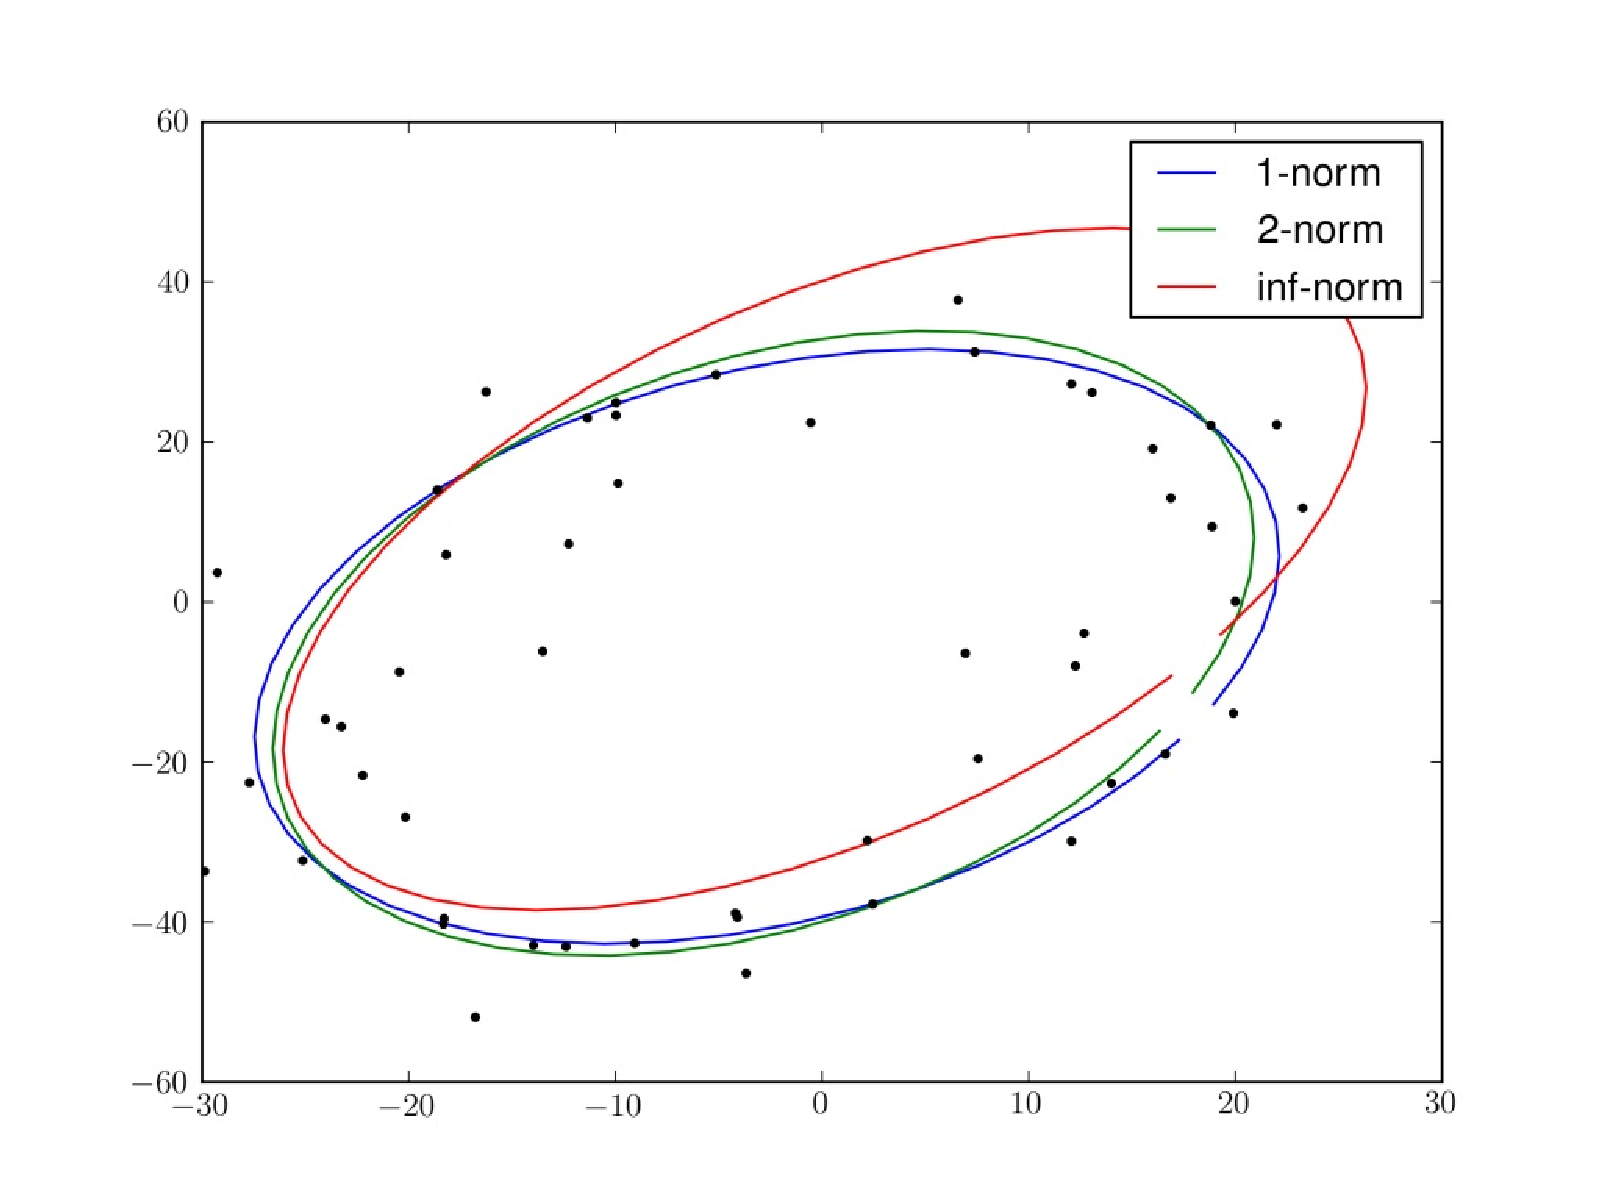
\includegraphics[width=\textwidth]{figures/ellipsefit.pdf}
\caption{Fitting an ellipse using different norms.}
\label{Fig:ellipse}
\end{figure}

\subsection*{Improvements to the QR Algorithm} % ------------------------------

\end{comment}
